% -*- compile-command: "make jss-slides.pdf" -*-
\documentclass{beamer}
\usepackage{tikz}
\usepackage[all]{xy}
\usepackage{amsmath,amssymb}
\usepackage{hyperref}
\usepackage{graphicx}
\usepackage{algorithmic}
\usepackage{multirow}

\DeclareMathOperator*{\argmin}{arg\,min}
\DeclareMathOperator*{\Lik}{Lik}
\DeclareMathOperator*{\PoissonLoss}{PoissonLoss}
\DeclareMathOperator*{\Peaks}{Peaks}
\DeclareMathOperator*{\Segments}{Segments}
\DeclareMathOperator*{\argmax}{arg\,max}
\DeclareMathOperator*{\maximize}{maximize}
\DeclareMathOperator*{\minimize}{minimize}
\newcommand{\sign}{\operatorname{sign}}
\newcommand{\RR}{\mathbb R}
\newcommand{\ZZ}{\mathbb Z}
\newcommand{\NN}{\mathbb N}
\newcommand{\z}{$z = 2, 4, 3, 5, 1$} 

\newcommand{\algo}[1]{\textcolor{#1}{#1}}
\definecolor{PDPA}{HTML}{66C2A5}
\definecolor{CDPA}{HTML}{FC8D62}
\definecolor{GPDPA}{HTML}{4D4D4D}

% Set transparency of non-highlighted sections in the table of
% contents slide.
\setbeamertemplate{section in toc shaded}[default][100]
\AtBeginSection[]
{
  \setbeamercolor{section in toc}{fg=red} 
  \setbeamercolor{section in toc shaded}{fg=black} 
  \begin{frame}
    \tableofcontents[currentsection]
  \end{frame}
}

\begin{document}

\title{Introducing Luke Tierney and Martin Maechler}

\author{
  Toby Dylan Hocking\\
  toby.hocking@nau.edu\\
  toby.hocking@r-project.org\\
}

\date{8 July 2020}

\maketitle

\begin{frame}[fragile]
  \frametitle{Top 10 committers to R project SVN repository}

  \begin{verbatim}
         author commits
 1:      ripley 37111
 2:    maechler 13563 <-
 3:      hornik  9100
 4:          pd  5604
 5:     murdoch  2884
 6:        luke  2182 <-
 7:         jmc   934
 8:       iacus   915
 9:      leisch   828
10:    kalibera   766
\end{verbatim}

  Source: \url{https://svn.r-project.org}, My analysis code:
  \url{https://github.com/tdhock/r-devel-emails}
  
\end{frame}

\begin{frame}
  \frametitle{Luke Tierney 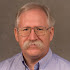
\includegraphics[height=2cm]{photo_luke}}

  \begin{itemize}
  \item Ralph E. Wareham Professor of Mathematical Sciences,
    Department of Statistics and Actuarial Science, University of
    Iowa, August 2002 -- Present
  \item Author of Lisp-Stat (amazing dynamic/interactive graphics).
  \item Joined R-core in 1998.
  \item Numerous contributions to R computational
    infrastructure (byte code compiler, ALTREP, memory management, ...)
  \item Encyclopedic knowledge of R internals. I've seen quite a few
    R-devel messages asking ``I think this weird R behavior is a
    bug---or is it intentional?'' to which Luke invariably replies
    something like ``Yes, to resolve
    \url{https://bugs.r-project.org/bugzilla/show_bug.cgi?id=15199}''
  \end{itemize}

  Sources: \url{https://stat.uiowa.edu/people/luke-tierney},
  \url{http://homepage.divms.uiowa.edu/~luke/}, Gmail photo
  
\end{frame}

\begin{frame}
  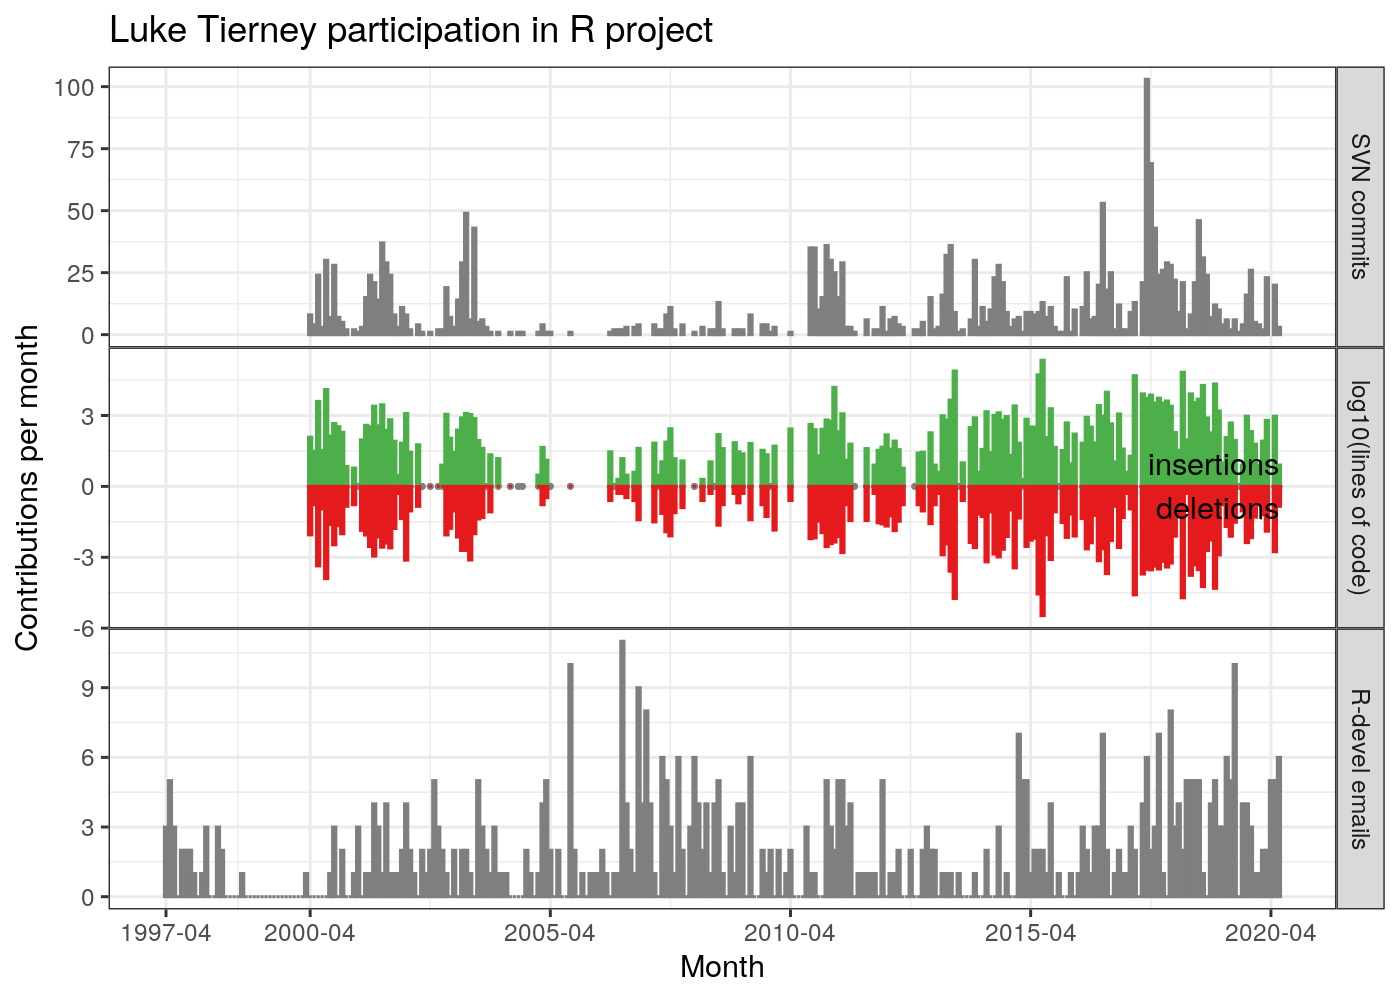
\includegraphics[width=\textwidth]{monthly_code_Luke_Tierney.png}

  Sources: \url{https://github.com/wch/r-source},
  \url{https://stat.ethz.ch/pipermail/r-devel}, My analysis code:
  \url{https://github.com/tdhock/r-devel-emails}
  
\end{frame}

\begin{frame}
  \frametitle{Martin Maechler 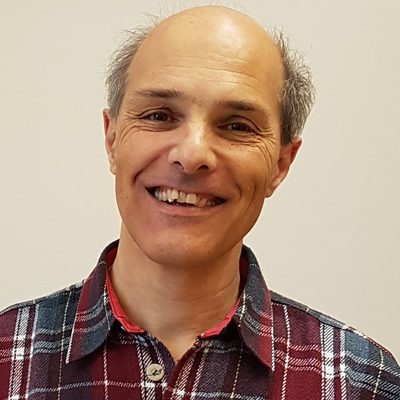
\includegraphics[height=2cm]{photo_martin}}

  \begin{itemize}
  \item Adjunct Professor at ETH Zurich.
  \item Joined R project in 1995, now R core team member.
  \item ESS Core dev since 1997, project lead since Aug 2004.
  \item Maintains recommended R package cluster.
  \item R task view on Robust statistical methods.
  \item Co-maintains R package Matrix.
  \item Manages the R stat.ethz.ch mailing lists.
  \item Invited talk at useR 2014.
  \item Gave me a bugzilla account on bugs.r-project.org
  \item R-project.org domain + email aliases.
  \end{itemize}

  Source: \url{https://stat.ethz.ch/~maechler/}
  
\end{frame}

\begin{frame}
  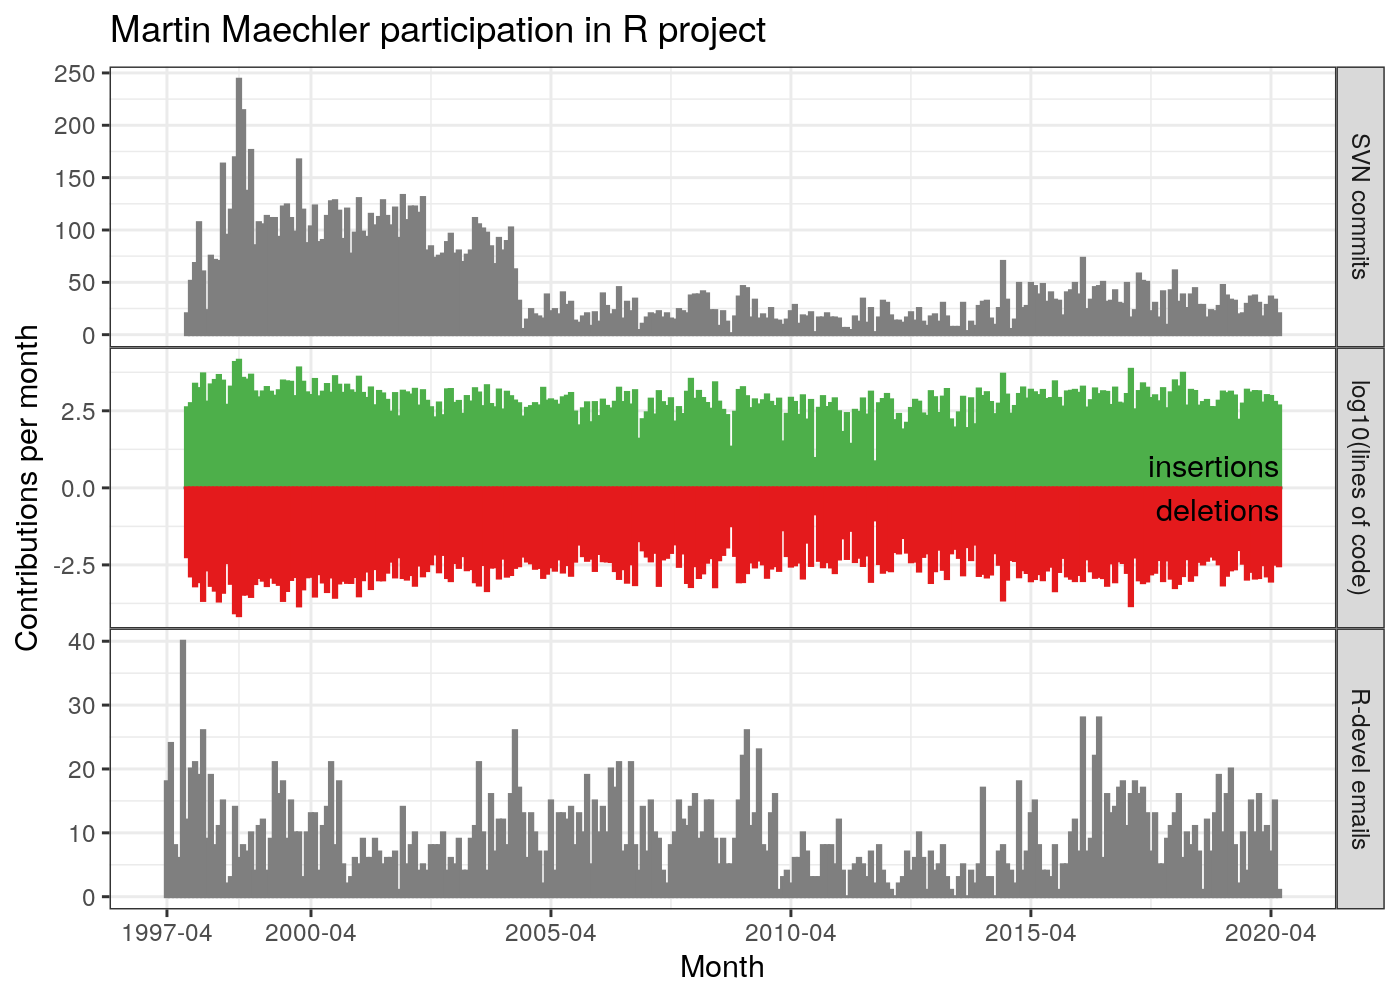
\includegraphics[width=\textwidth]{monthly_code_Martin_Maechler.png}
  
  Sources: \url{https://github.com/wch/r-source},
  \url{https://stat.ethz.ch/pipermail/r-devel}, My analysis code:
  \url{https://github.com/tdhock/r-devel-emails}
  
\end{frame}

\end{document}
